After the model construction verification was carried out to determine whether the model correctly implemented the calculations of the modified Newtonian method. This was done by placing two triangular surface elements in a flow. First at an angle and secondly normal to the flow. The model outputs were verified by also calculating the results by hand.

Following the verification process the model was validated using experimental values of different parameters. Each separate validation case will be treated here.

\subsubsection{\gls{sym:CD}-validation against experimental drag of a sphere}
\label{subsubsec:valsphere}
For the first model validation case a comparison was made the between the \gls{sym:CD}-value of a sphere in hypersonic flow that were computed by the model and as found in an experiment. It was found that for hypersonic Mach numbers the experimental \gls{sym:CD}-value of a sphere is $0.92$ \cite{Bailey1966,AndersonJr.2007,Cox1965}. When computing \gls{sym:CD} numerically with the modified Newtonian method using more than $10,000$ surface elements produces $\gls{sym:CD}=0.916$, which coincides with a discrepancy of $0.5\%$ of the experimental value. Since the accuracy of the experimental data is approximately $\pm1.5\%$ \cite{Bailey1966} this discrepancy falls within the confidence interval of the measurements.

\subsubsection{\gls{sym:CP}-validation against experimental data of a sharp cone}
\label{subsubsec:valsharpconeCP}
Following the \gls{sym:CD}-validation for blunt bodies presented in the previous section now \gls{sym:CP}-validation will be carried out for sharp bodies. This is performed by comparing \gls{sym:CP} at select points on the surface of a cone with half-cone angle \gls{sym:theta} of $15$ degrees. The experimental data was collected for $\gls{sym:M}=14.9$ and $\gls{sym:gamma}=\frac{5}{3}$  \cite{Bertin1994,Cleary1970}. Figure \ref{fig:CPcone30val} shows the data points that were collected for angles of attack $\gls{sym:alpha}=10[\deg]]$ and $\gls{sym:alpha}=20[\deg]$ in Figure \ref{fig:CPconealpha10} and \ref{fig:CPconealpha20} respectively. On the X-axis the variable \gls{sym:beta_cone} is used. This quantity refers to the local cross-sectional surface rotation with respect to an axis that is defined positive in the positive Z-direction. Figure \ref{fig:beta_cone} showcases this concept more clearly. Normally the domain of \gls{sym:beta_cone} lies between $0[\deg]$ and $360[\deg]$, but because the cone is symmetrical only half of the cone surface is plotted here. Furthermore, since the cone in question is a sharp cone with a constant semi-cone angle the \gls{sym:CP}-distribution is constant along the cone surface for constant \gls{sym:beta_cone}.
As can be seen in Figures \ref{fig:CPconealpha10} and \ref{fig:CPconealpha20} the modified Newtonian method is the most accurate around $\gls{sym:beta_cone}=90[\deg]$.

\begin{figure}[ht]
	\centering
	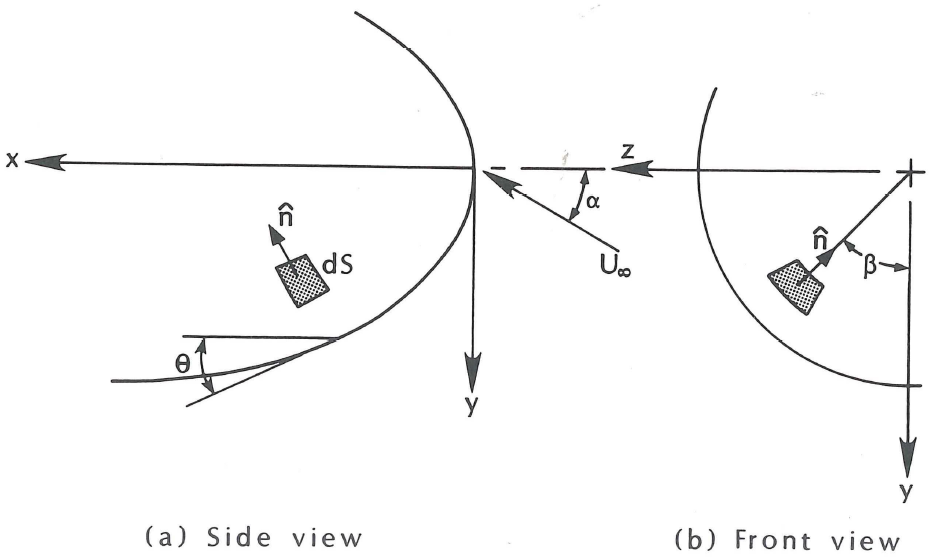
\includegraphics[width=0.7\textwidth]{./Figure/Aerodynamics/def_beta}
	\caption[Definition of \gls{sym:beta_cone}]{Definition of \gls{sym:beta_cone} \cite{Bertin1994}}
	\label{fig:beta_cone}
\end{figure}

\begin{figure}[ht]
	\centering
	\begin{subfigure}[b]{0.49\textwidth}
		\centering
		\setlength\figureheight{0.6\textwidth} 
		\setlength\figurewidth{0.85\textwidth}
		% This file was created by matlab2tikz.
% Minimal pgfplots version: 1.3
%
\definecolor{mycolor1}{rgb}{0.20810,0.16630,0.52920}%
\definecolor{mycolor2}{rgb}{0.19855,0.72140,0.63095}%
%
\begin{tikzpicture}

\begin{axis}[%
width=0.95092\figurewidth,
height=\figureheight,
at={(0\figurewidth,0\figureheight)},
scale only axis,
xmin=0,
xmax=200,
xlabel={$\beta$ [deg]},
xmajorgrids,
ymin=0,
ymax=0.4,
ylabel={$C_p$ [-]},
ymajorgrids,
legend style={legend cell align=left,align=left,draw=white!15!black}
]
\addplot [color=mycolor1,solid]
  table[row sep=crcr]{%
0	0.313663919882391\\
4.55696202531646	0.312877849005529\\
9.11392405063291	0.310530499749308\\
13.6708860759494	0.306654244746176\\
18.2278481012658	0.301302318547099\\
22.7848101265823	0.29454775570286\\
27.3417721518987	0.286481939294681\\
31.8987341772152	0.277212794080603\\
36.4556962025316	0.266862666715091\\
41.0126582278481	0.255565942738302\\
45.5696202531646	0.243466456039843\\
50.126582278481	0.230714751131957\\
54.6835443037975	0.217465261705828\\
59.2405063291139	0.203873470516536\\
63.7974683544304	0.190093115610837\\
68.3544303797468	0.176273506281338\\
72.9113924050633	0.162557008944947\\
77.4683544303798	0.14907675848562\\
82.0253164556962	0.135954644591526\\
86.5822784810127	0.123299615408348\\
91.1392405063291	0.111206332607406\\
95.6962025316456	0.0997542029384269\\
100.253164556962	0.0890068017311918\\
104.810126582279	0.0790116938710017\\
109.367088607595	0.0698006477512688\\
113.924050632911	0.0613902278554033\\
118.481012658228	0.0537827421878944\\
123.037974683544	0.046967511998371\\
127.594936708861	0.0409224233429402\\
132.151898734177	0.0356157132021625\\
136.708860759494	0.0310079372951395\\
141.26582278481	0.0270540625330662\\
145.822784810127	0.023705624346723\\
150.379746835443	0.0209128879663695\\
154.93670886076	0.0186269531555022\\
159.493670886076	0.016801743887958\\
164.050632911392	0.0153958279571552\\
168.607594936709	0.0143740164247398\\
173.164556962025	0.0137086990254263\\
177.721518987342	0.0133808789844762\\
182.278481012658	0.0133808789844762\\
};
\addlegendentry{Modified Newtonian};

\addplot [color=mycolor2,only marks,mark=asterisk,mark options={solid}]
  table[row sep=crcr]{%
0	0.359\\
30	0.326\\
60	0.234\\
90	0.112\\
120	0.06\\
150	0.037\\
180	0.039\\
};
\addlegendentry{Measured};

\end{axis}
\end{tikzpicture}%
		\caption{$\gls{sym:alpha}=10\deg$}
		\label{fig:CPconealpha10}
	\end{subfigure}
		\begin{subfigure}[b]{0.49\textwidth}
			\centering
			\setlength\figureheight{0.6\textwidth} 
			\setlength\figurewidth{0.85\textwidth}
			% This file was created by matlab2tikz.
% Minimal pgfplots version: 1.3
%
\definecolor{mycolor1}{rgb}{0.20810,0.16630,0.52920}%
\definecolor{mycolor2}{rgb}{0.19855,0.72140,0.63095}%
%
\begin{tikzpicture}

\begin{axis}[%
width=0.95092\figurewidth,
height=\figureheight,
at={(0\figurewidth,0\figureheight)},
scale only axis,
xmin=0,
xmax=200,
xlabel={$\beta$ [deg]},
xmajorgrids,
ymin=0,
ymax=0.7,
ylabel={$C_p$ [-]},
ymajorgrids,
legend style={legend cell align=left,align=left,draw=white!15!black}
]
\addplot [color=mycolor1,solid]
  table[row sep=crcr]{%
0	0.577764228354504\\
4.55696202531646	0.575664128443356\\
9.11392405063291	0.569399969689605\\
13.6708860759494	0.559079369250394\\
18.2278481012658	0.544879022785013\\
22.7848101265823	0.527040773405377\\
27.3417721518987	0.505866243155278\\
31.8987341772152	0.481710157904938\\
36.4556962025316	0.454972528255649\\
41.0126582278481	0.426089876689746\\
45.5696202531646	0.395525724083726\\
50.126582278481	0.363760566256924\\
54.6835443037975	0.331281583018694\\
59.2405063291139	0.298572327912705\\
63.7974683544304	0.26610264639941\\
68.3544303797468	0.234319063584449\\
72.9113924050633	0.203635869964691\\
77.4683544303798	0.174427115348786\\
82.0253164556962	0.1470196975823\\
86.5822784810127	0.121687704566509\\
91.1392405063291	0.0986481360184979\\
95.6962025316456	0.0780580962897468\\
100.253164556962	0.0600135122299421\\
104.810126582279	0.044549391495899\\
109.367088607595	0.0316415978371448\\
113.924050632911	0.0212100817210665\\
118.481012658228	0.0131234681544689\\
123.037974683544	0.00720486963515046\\
127.594936708861	0.00323876168105333\\
132.151898734177	0.000978732102579191\\
136.708860759494	0.000121379574901702\\
141.26582278481	0\\
145.822784810127	0\\
150.379746835443	0\\
154.93670886076	0\\
159.493670886076	0\\
164.050632911392	0\\
168.607594936709	0\\
173.164556962025	0\\
177.721518987342	0\\
182.278481012658	0\\
};
\addlegendentry{Modified Newtonian};

\addplot [color=mycolor2,only marks,mark=asterisk,mark options={solid}]
  table[row sep=crcr]{%
0	0.63\\
30	0.55\\
60	0.327\\
90	0.093\\
120	0.028\\
150	0.009\\
180	0.014\\
};
\addlegendentry{Measured};

\end{axis}
\end{tikzpicture}%
		\caption{$\gls{sym:alpha}=20\deg$}
		\label{fig:CPconealpha20}
	\end{subfigure}
	\caption{Comparisons between experimental and numerical pressure coefficients}
	\label{fig:CPcone30val}
\end{figure}

\subsubsection{\gls{sym:CD}-validation against experimental data of a sharp cone}
\label{subsubsec:valsharpconeCD}
Stevens found that for a sharp cone-cylinder with half-cone angle \gls{sym:theta} of $30\deg$ $\gls{sym:CD}=0.58$ in an air-stream of Mach $8$ where angle of attack \gls{sym:alpha} and sideslip angle \gls{sym:beta} are zero \cite{Stevens1950,AndersonJr.2007}. The numerical model predicts for this case that $\gls{sym:CD}=0.456$, which coincides with a discrepancy of $21.4\%$ of the experimental value. This is in line with the results of section \ref{subsubsec:valsharpconeCP} where the \glspl{sym:CP} predicted by the numerical model were smaller than the experimental values of a sharp cone.

\subsubsection{\gls{sym:CP}-validation against experimental data of the Apollo re-entry capsule}
\label{subsubsec:Apollo_validation}
The data points in Figure \ref{fig:Apollo_cp} represent pressure coefficients measured at various locations of one of the two axisymmetric axes \cite{Bertin1966}. The quantity shown on the X-axis is defined in Figure \ref{fig:Apollo_y}. As can be seen in Figure \ref{fig:Apollo_cp} the numerical model is most accurate around the centre of the capsule. As the distance to the centreline increases, so does the discrepancy between the experimental and numerical values.

\begin{figure}[ht]
	\centering
	\setlength\figureheight{0.4\textwidth} 
	\setlength\figurewidth{0.95\textwidth}
	% This file was created by matlab2tikz.
% Minimal pgfplots version: 1.3
%
\definecolor{mycolor1}{rgb}{0.20810,0.16630,0.52920}%
\definecolor{mycolor2}{rgb}{0.19855,0.72140,0.63095}%
%
\begin{tikzpicture}

\begin{axis}[%
width=0.95092\figurewidth,
height=\figureheight,
at={(0\figurewidth,0\figureheight)},
scale only axis,
unbounded coords=jump,
xmin=-1.5,
xmax=1.5,
xlabel={$\frac{s}{R}$ [-]},
xmajorgrids,
ymin=0,
ymax=1.8,
ylabel={$C_p$ [-]},
ymajorgrids,
legend style={at={(0.5,0.03)},anchor=south,legend cell align=left,align=left,draw=white!15!black}
]
\addplot [color=mycolor1,solid]
  table[row sep=crcr]{%
-1.095	0.00194223338446491\\
-1.09496992147514	0\\
-1.09472939221993	0.0105764109659139\\
-1.09463923908848	0\\
-1.09415883985204	0.0286612804702033\\
-1.09400885921748	0\\
-1.09328990674072	0.0560242775566994\\
-1.09308050968954	0\\
-1.09212497457122	0.092367937353207\\
-1.09185673504618	0\\
-1.09066723634165	0.137297047773714\\
-1.09034088956864	0\\
-1.08892068761116	0.190322850013229\\
-1.08853712808401	0\\
-1.08689011554844	0.250868241388263\\
-1.08645039457714	nan\\
-1.08458108581034	0.318273930108563\\
-1.0819999272869	0.3918054818373\\
-1.07915371475421	0.470661188513422\\
-1.07605024948299	0.55398068095838\\
-1.07269803785581	0.640854198362098\\
-1.06910626805175	0.730332419944821\\
-1.06528478486218	0.821436757031353\\
-1.06124406270688	0.913169997566455\\
-1.05699517692443	1.00452718986455\\
-1.05254977341541	1.09450664823589\\
-1.04792003672184	1.18212096017887\\
-1.0431186566302	1.26640787317747\\
-1.03815879338958	1.34644093888065\\
-1.03305404164036	1.42133979364298\\
-1.02781839315226	1.42835417521564\\
-1.01832656548985	1.44935521736688\\
-0.986104624404206	1.50751538767456\\
-0.953709183690762	1.52351962805163\\
-0.921145943147255	1.5390688207566\\
-0.888420632094868	1.55415195599687\\
-0.855539008370191	1.56875835245074\\
-0.822506857312158	1.58287766497233\\
-0.789329990744154	1.59649989205813\\
-0.75601424595145	1.60961538306931\\
-0.72256548465417	1.62221484520418\\
-0.688989591975953	1.63428935021542\\
-0.655292475408497	1.64583034086682\\
-0.621480063772172	1.6568296371244\\
-0.587558306172872	1.66727944207735\\
-0.553533170955306	1.67717234758383\\
-0.519410644652901	1.68650133963741\\
-0.485196730934503	1.69525980344988\\
-0.450897449548067	1.7034415282464\\
-0.416518835261513	1.71104071176934\\
-0.382066936800948	1.71805196448708\\
-0.347547815786417	1.72447031350459\\
-0.312967545665402	1.7302912061727\\
-0.27833221064423	1.73551051339311\\
-0.243647904617593	1.74012453261658\\
-0.208920730096357	1.74412999053202\\
-0.174156797133862	1.74752404544416\\
-0.139362222250891	1.7503042893381\\
-0.104543127359504	1.75246874962895\\
-0.0697056386859186	1.75401589059533\\
-0.0348558856926369	1.75488268492153\\
-0	1.75525426236477\\
0.0348558856926369	1.75488268492153\\
0.0697056386859186	1.75401589059533\\
0.104543127359504	1.75246874962895\\
0.139362222250891	1.7503042893381\\
0.174156797133862	1.74752404544416\\
0.208920730096357	1.74412999053202\\
0.243647904617593	1.74012453261658\\
0.27833221064423	1.73551051339311\\
0.312967545665402	1.7302912061727\\
0.347547815786417	1.72447031350459\\
0.382066936800948	1.71805196448708\\
0.416518835261513	1.71104071176934\\
0.450897449548067	1.7034415282464\\
0.485196730934503	1.69525980344988\\
0.519410644652901	1.68650133963741\\
0.553533170955306	1.67717234758383\\
0.587558306172872	1.66727944207735\\
0.621480063772172	1.6568296371244\\
0.655292475408497	1.64583034086682\\
0.688989591975953	1.63428935021542\\
0.72256548465417	1.62221484520418\\
0.75601424595145	1.60961538306931\\
0.789329990744154	1.59649989205813\\
0.822506857312158	1.58287766497233\\
0.855539008370191	1.56875835245074\\
0.888420632094868	1.55415195599687\\
0.921145943147255	1.5390688207566\\
0.953709183690762	1.52351962805163\\
0.986104624404206	1.50751538767456\\
1.01832656548985	1.44935521736688\\
1.02781839315226	1.42835417521564\\
1.03305404164036	1.42133979364298\\
1.03815879338958	1.34644093888065\\
1.0431186566302	1.26640787317747\\
1.04792003672184	1.18212096017886\\
1.05254977341541	1.09450664823589\\
1.05699517692443	1.00452718986455\\
1.06124406270688	0.913169997566455\\
1.06528478486218	0.821436757031353\\
1.06910626805175	0.730332419944821\\
1.07269803785581	0.640854198362098\\
1.07605024948299	0.55398068095838\\
1.07915371475421	0.470661188513422\\
1.0819999272869	0.3918054818373\\
1.08458108581034	0.318273930108563\\
1.08645039457714	nan\\
1.08689011554844	0.250868241388263\\
1.08853712808401	0\\
1.08892068761116	0.190322850013229\\
1.09034088956864	0\\
1.09066723634165	0.137297047773714\\
1.09185673504618	0\\
1.09212497457122	0.0923679373532069\\
1.09308050968954	0\\
1.09328990674072	0.0560242775566994\\
1.09400885921748	0\\
1.09415883985204	0.0286612804702033\\
1.09463923908848	0\\
1.09472939221993	0.0105764109659139\\
1.09496992147514	0\\
1.095	0.0019422333844649\\
};
\addlegendentry{Modified Newtonian};

\addplot [color=mycolor2,only marks,mark=asterisk,mark options={solid}]
  table[row sep=crcr]{%
-1.02718093698553	0.326751322056051\\
-0.951551131339198	1.02168543257076\\
-0.799264139197169	1.4880212545932\\
-0.247616441864002	1.7300201625693\\
0.0180691662280614	1.74873159897289\\
0.273850147488554	1.70299372722051\\
0.547682381293604	1.63105638244619\\
0.68183629061674	1.49350323432687\\
0.817930550476365	1.44043342939967\\
0.871460439771112	1.37207156639853\\
0.929404854806911	1.26182928317321\\
0.981710021888355	0.939565894363321\\
1.0408671541418	0.31807000221393\\
1.09530512997895	0.0391870122023066\\
};
\addlegendentry{Measured};

\end{axis}
\end{tikzpicture}%
	\caption{Comparison between experimental and numerical \glspl{sym:CP} for the Apollo re-entry capsule}
	\label{fig:Apollo_cp}
\end{figure}

\begin{figure}[ht]
	\centering
	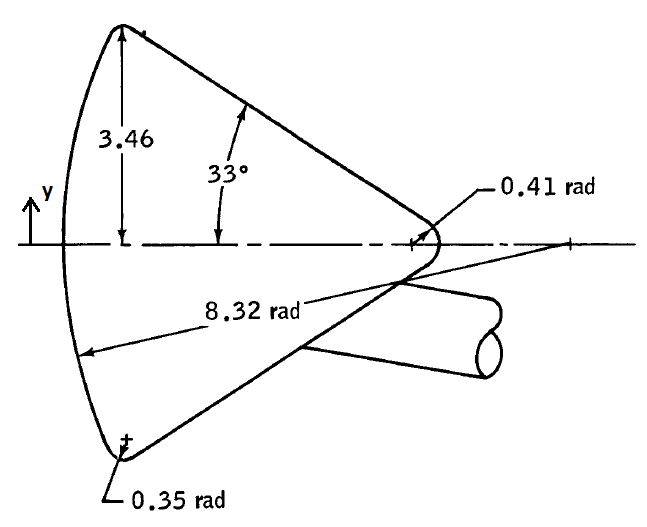
\includegraphics[width=0.4\textwidth]{./Figure/Aerodynamics/Apollo_model}
	\caption[Definition of unit on the horizontal axis of Figure \ref{fig:Apollo_cp}]{Definition of unit on the horizontal axis of Figure \ref{fig:Apollo_cp} \cite{Bertin1966}}
	\label{fig:Apollo_y}
\end{figure}

\subsubsection{Maximum heat flux validation against experimental data of the \gls{irve} 3 vehicle}
\label{subsubsec:heatvalidation}
Dillman et al. observed that the maximum heat flux on the \acrfull{irve} 3 was $14.4$ $[W\cdot cm^{-2}]$ during re-entry at an altitude of $50$ kilometres and Mach $7.0$ \cite{Dillman2012}. The maximum heat flux computed by the numerical tool in the stagnation point for these flow conditions is $11.7$ $[W\cdot cm^{-2}]$. This is equal to $81.0\%$ of the experimental value. Thus a discrepancy of $19.0\%$ is present between the experimental and numerical maximum heat fluxes.

\subsubsection{Conclusions after the validation procedure}
\label{subsec:validconclusions}
From the previous sections it can be seen that the accuracy of the modified Newtonian method varies between geometries. The \gls{sym:CD} predicted in section \ref{subsubsec:valsphere} is accurate to within $1\%$ of the experimental value, whereas the accuracy of the \glspl{sym:CP} in section \ref{subsubsec:valsharpconeCP} varied over the cone surface. This discrepancy was also seen in section \ref{subsubsec:valsharpconeCD}, where the difference between the numerical and experimental \gls{sym:CD} was $21.4\%$, and again for the Apollo capsule in section \ref{subsubsec:Apollo_validation}. These discrepancies are expected, as the Modified Newtonian flow theory is only valid when pressure drag dominates the total drag. At lower incidence angles with the flow, this situation no longer holds. The estimated pressure coefficients are therefore incorrect at high incidence angles. This can be seen around the edges of the Apollo re-entry capsule and on the surface of the sharp cone, where the discrepancies are largest.  

 After judging the accuracy shown in Figures \ref{fig:CPcone30val} and \ref{fig:Apollo_cp} it was determined that the accuracy of the modified Newtonian method is adequate for the conceptual and preliminary design phases, since the body will be a blunt body at low to moderate incidence angles to the flow. The body therefore operates within the useful range of modified Newtonian flow theory. 
The model for the maximum heat flux found on a body was validated in section \ref{subsubsec:heatvalidation}. It was observed that a discrepancy of $19.0\%$ was present between the numerical and experimental maximum heat fluxes. Possible causes for this discrepancy lie in the difference between the atmospheric conditions at the time of the measurement during the \gls{irve} mission and the international standard atmosphere and in the fact that the theory used is an empirical method which is not an exact expression for the heat flux derived from governing flow equations.  After consideration this was deemed to be acceptable for conceptual and preliminary design.